\documentclass[11pt,a4paper]{amsart}

\usepackage{amssymb}
\usepackage{geometry}
\usepackage{commath}
\usepackage{dsfont}
\usepackage{enumerate}
\usepackage{graphicx}
\usepackage{todonotes}
\geometry{margin=2.5cm}
%\setlength{\parindent}{0pt}

\newtheorem*{problem}{Problem}
\theoremstyle{definition}
\newtheorem*{answer}{Answer}
\DeclareMathOperator{\supp}{supp}
\DeclareMathOperator{\ran}{ran}
\DeclareMathOperator{\dom}{dom}
\DeclareMathOperator{\spann}{span}
\DeclareMathOperator{\col}{col}
\DeclareMathOperator{\row}{row}
\DeclareMathOperator{\Id}{Id}
\renewcommand{\span}{\spann}
\newcommand{\bbone}{\mathds{1}}
\begin{document}

\title{A first implementation of Section 3 of ``Bla Parabolic''}
\author{Jan Westerdiep}
\maketitle

I've spent the past two weeks on a (not yet) linear time implementation of \S 3
from ``Bla Parabolic''. Currently it can only apply multiscale (mass) operator
in the time direction; I felt it was better to have a good understanding of one
aspect than to produce a half-baked implementation for the tensor-product case.

\subsection*{A little bit on notation} I am somewhat hesitant to call these
`mass matrices' \emph{matrices} because this implies that the rows and columns
are ordered, whereas we have mere \emph{sets} of indices (which are not necessarily
ordered). I will try to call everything \emph{linear operators} from one
\emph{vector space} to another, instead of matrices working on vectors.

The vector spaces that we will be working with are often sequence spaces
$\ell_2(\Lambda)$ for some finite index set $\Lambda$. If we were to order this
index set in, say, lexicographic ordering, then $\ell_2(\Lambda)$ corresponds
directly with $\mathbb{R}^{\# \Lambda}$.

\section{The Applicator}
The meat of the algorithm is in \texttt{applicator.py}. This \texttt{Applicator}
class has a constructor which takes, at minimum, a \texttt{Basis} object
$B = \Phi \cup \Psi$ and a singlescale \texttt{LinearOperator} object
$\mathcal A: \span \Phi \to (\span \Phi)'$. Both $\Phi$ and $\Psi$ are indexed by
\texttt{IndexSets}, with $\Phi$ indexed by a list of \texttt{SingleLevelIndexSet}s
$\Delta_\ell$ and $\Psi$ by a \texttt{MultiScaleIndexSet} (or \emph{tree})
which we call $\Lambda$. Remember that by assumption $\span \Phi = \span \Psi$.
It is also possible to construct the \texttt{Applicator} with different in- and
out-bases when the domain and range of $\mathcal A$ do not coincide.

It has three public methods: \texttt{apply()}, \texttt{apply\_upp()},
and \texttt{apply\_low()}. These methods in turn invoke recursive methods that
traverse $\Lambda$, starting from level $\ell=1$ until its maximum level, at
each level applying $\mathcal A$ to a subset of the singlescale indices
$\Delta_\ell$ on level $\ell$. In doing this, it needs the \texttt{SLIS}s
$\check \Pi_B^\ell := \check \Pi_B$ (named \texttt{Pi\_B\_out} in the code
corresponding with the out-basis), $\Pi_B^\ell = \Pi_B$ named
\texttt{Pi\_B\_in}, $\underline \Pi^\ell = \Pi^{\ell + 1}$ named \texttt{Pi\_bar\_in},
and $\underline{\check \Pi}^\ell = \check \Pi^{\ell+1}$. It is important to note 
that even when $\ran \mathcal A = \dom \mathcal A$, in general $\check \Pi_B \not= \Pi_B$
and hence $\underline{\check \Pi} \not= \underline \Pi$.

Computing these subsets $\check \Pi_B, \Pi_B, \underline{\check \Pi}, \underline \Pi$
in linear time is not an easy task. I was able to produce them in suboptimal complexity;
see the code. Maybe Rob will have an idea on how to tackle these.

\subsection{Constructing $\Pi_B$}
I am not \emph{at all} sure what $\Pi_B$ is supposed to do, but I feel like it's
the set of indices that are supposed to be lifted to level $\ell+1$. I computed 
\[
  \Pi_B := \set{\lambda \in \Pi: |\supp \phi_\lambda \cap
      (\cup_{\mu \in \check \Lambda_\ell} \supp \check \psi_\mu
       \cup_{\gamma \in \check \Pi_B} \supp \check \phi_\gamma)| > 0}
\]
by collecting all these supports $[a,b]$, sorting them\footnote{Blehhhh; see code
for a justification and a possible solution; still, this doesn't reduce the
operation to optimal complexity.} in order of increasing $a$, and merging them
pairwise to a minimum-size \texttt{IntervalSet} that covers the same intervals
as the original supports. We can loop over all $\lambda \in \Pi$ and check if
this \texttt{IntervalSet} \texttt{intersects()} its support. This is possibly
$\mathcal O[\# \Pi_B (\# \Lambda_\ell + \# \check \Pi_B) \log(\# \Lambda_\ell + \# \check \Pi_B)]$
operations where we would like $\mathcal O(\# \Pi_B$).  In practice though,
$\#\mathtt{IntervalSet} \ll \# \Lambda_\ell + \# \check \Pi_B$, so this helps
\emph{a lot} for faster runtimes.

On the other
hand $\Pi_A := \Pi \setminus \Pi_B$ is the set of indices we will want restrict
the result of applying $\mathcal A$ to, and these will not be lifted to the next
level. In Kestlers C++-code, (the equivalent of) $\Pi_A$ rather than $\Pi_B$ is
computed. This may be a way of doing it in linear time?

\subsection{Constructing $\underline \Pi$}
The construction of $\underline \Pi$ is very similar to the previous method, the
big difference being that we want to collect those indices $\lambda \in \Delta_\ell$
that are completely covered by the \texttt{IntervalSet}.

\subsection{Applying $P^\ell$ and $Q^\ell$, and restriction of vectors to subsets}
Throughout the algorithm, it is necessary to restrict a vector to a subset of
indices, e.g.
\[
  \underline{\vec d} := (P^\ell \vec d|_{\Pi_B} + Q^\ell \vec c|_{\Lambda_\ell})|_{\underline \Pi}.
\]
Instead of manually setting vector indices to zero, computing the result of the
linear operator on the full set $\Delta_{\ell + 1}$ and then again setting vector
indices to zero, instead we compute the result of the \texttt{LinearOperator}s
$P^\ell$ and $Q^\ell$ only on those indices in $\underline \Pi$, and in the inner
products of rows of the \texttt{LinearOperator} with the \texttt{IndexedVector},
we only consider those indices in $\Pi_B$ resp.~$\Lambda_\ell$, thus effectively
`zero-ing out' the other indices. We know that every
row of $P^\ell$ and $Q^\ell$ have $\lesssim 1$ number of nonzeros, so this inner
product can be computed in $O(1)$ operations.\footnote{One actually has to take
care in not looping over elements in $\Pi_B$ to see if the corresponding cell in
$P^\ell$ is nonzero, but rather loop over nonzeros in $P^\ell$ to see if they
are in $\Pi_B$. This mistake destroyed linearity at first, and took me quite some
time to fix.}

The linear operators $P^\ell$ and $Q^\ell$ are the unique ones such that
\[
  \Phi_{\ell-1}^\top = \Phi_\ell^\top P^\ell, \quad \Psi_\ell^\top = \Phi_\ell^\top Q^\ell.
\]
These exist because $\span \Phi_{\ell-1} \subset \span \Phi_\ell$ and
$\span \Psi_\ell \subset \span \Phi_\ell$ by assumption. For some $\phi_\lambda \in \Phi_{\ell-1}$,
we see that $\Phi_\ell^\top p_{\ell,\lambda}$: the linear operator $P^\ell$ gives us the
coefficients necessary to build a scaling function on the previous level using
scaling functions on this level: a little more on this later. Similar equalities
hold for the $Q^\ell$.

We also have to apply the transpose of $P^\ell$ and $Q^\ell$; building these
efficiently proved to be quite the obstacle for the more esoteric 3-point basis.

\subsection{Summation of vectors}
There is a number of places in the \texttt{Applicator} where vectors are built
by stacking multiple vectors indexed by disjoint sets (e.g.~$\vec e$ and $\vec f$).
We can be lazy and just write these as the sum of the two vectors.

\section{Bases}
In this proof-of-concept application, we will work with three bases: the Haar
basis, the orthonormal discontinuous piecewise linear basis, and the three-point
hierarchical basis. Every basis contains a \emph{singlescale} or \emph{scaling
basis} $\Phi$ indexed on every level by $\Delta_\ell$, and a \emph{multiscale}
or \emph{wavelet basis} $\Psi$ indexed by a tree $\Lambda$. Every index $lambda$
is a tuple $(\ell, n)$; its level and its \emph{offset}, even though in the
multiwavelet/multiscaling case, the offset also determines \emph{which} mother
scaling function $\phi_\lambda$ descends from.

Every \texttt{Basis} object is constructed by passing it the \texttt{MultiScaleIndexSet}
$\Lambda$. Upon construction, it exposes as properties the \texttt{LinearOperator}s
$P := (P^\ell)_{\ell}$ and $Q = (Q^\ell)_\ell$, as well as one or more singlescale
\texttt{LinearOperator}s like the mass and \emph{damping} operators
\[
  (M\Phi_\ell)(\Phi_\ell) := \left[\int_0^1 \phi_\lambda \phi_\mu \dif t \right]_{\lambda,\mu \in \Delta_\ell}, \quad
  (C\Phi_\ell)(\Phi_\ell) := \left[\int_0^1 \phi_\lambda' \phi_\mu \dif t \right]_{\lambda,\mu \in \Delta_\ell}.
\]

It has methods to compute the support of scaling- and wavelet functions (with
\texttt{Interval} return types), as well as the \emph{wavelet neighbourhood}
$S(\mu) \supset \supp \psi_\mu$ (which, for all our cases, just equals the support).

\subsection{Singlescale matrices}
I basically just computed the singlescale matrices using pen and paper or
Mathematica.

\subsection{$P^\ell$ and $Q^\ell$}
In general, the following equalities define $P^\ell$ and $Q^\ell$:
\[
\begin{cases}
  \phi_\lambda := \langle\Phi_\ell, \col_\lambda(P^\ell)\rangle_{\ell_2(\Delta_\ell)} = \sum_{\mu \in \Delta_\ell} P^\ell_{\mu,\lambda} \phi_\mu & \lambda \in \Delta_{\ell-1},\\
  \psi_\lambda := \langle \Phi_{\ell}, \col_\lambda(Q^\ell)\rangle_{\ell_2(\Delta_\ell)} = \sum_{\mu \in \Delta_\ell} Q^\ell_{\mu,\lambda} \phi_\mu & \lambda \in \Lambda_\ell.
\end{cases}
\]
This means that $P^\ell$ tells us exactly how to write a scaling function on the
previous level in terms of scaling functions on the current level, and that $Q^\ell$
tells us how to write wavelet functions on this level in terms of scaling functions
on this level.

\subsubsection*{Haar basis}
The Haar basis has mother scaling resp.~wavelet functions
\[
  \phi(x) := \bbone_{[0,1)}(x), \quad \psi(x) := \bbone_{[0,\frac{1}{2})}(x) - \bbone_{[\frac{1}{2},1)}(x).
\]
At index $\lambda = (\ell, n)$, we have
\[
  \phi_\lambda(x) = \phi(2^\ell x - n), \quad \psi_\lambda(x) = \psi(2^{\ell-1}x - n).
\]
This $2^\ell$ versus $2^{\ell-1}$ is to balance the assumption that on level 0,
$\Psi_0 = \Phi_0$ (so that the mother wavelet function actually lives on level 1,
whereas the mother scaling function lives on level 0).

The result is that for the Haar basis, both $P$ and $Q$ have very simple structure:
\[
  \phi_\lambda = \phi_{(\ell+1, 2n)} + \phi_{(\ell+1, 2n+1)}, \quad
  \psi_\lambda = \phi_{(\ell, 2n)} - \phi_{(\ell, 2n+1)}.
\]
In other words, every column of $P^\ell$ and $Q^\ell$ has two nonzeros. If we
were to take all indices $\Lambda_\ell = (\ell, n)$ with $0 \leq n < 2^l$ and
order them in lexicographic ordering, then
\[
  P^{\ell} = \begin{bmatrix}1 \\ 1\end{bmatrix} \otimes \Id_{\ell}, \quad Q^{\ell} = \begin{bmatrix}1 \\ -1\end{bmatrix} \otimes \Id_{\ell}.
\]

\subsubsection*{Orthonormal basis}
The orthonormal discontinuous piecewise linear basis is a multiscaling/multiwavelet basis and has mother scaling functions
\[
  \phi_0(x) := \bbone_{[0,1)}(x), \quad \phi_1(x) := \sqrt{3} (2x-1) \bbone_{[0,1)}(x)
\]
with mother wavelet functions
\[
  \begin{cases}
    \psi_0(x) := (1-6x) \bbone_{[0,\frac{1}{2})}(x) + (5-6x)\bbone_{[\frac{1}{2},1)}(x), \\
    \psi_1(x) := \sqrt{3} (1-4x) \bbone_{[0,\frac{1}{2})}(x) + \sqrt{3}(4x-3)\bbone_{[\frac{1}{2},1)}(x)
  \end{cases}
\]
(see also the document by Rob for a more visual approach). We have
\[
  \phi_{(\ell, 2n)}(x) := \phi_0(2^\ell x - n), \quad \phi_{(\ell, 2n+1)}(x) := \phi_1(2^\ell x - n) \quad (\ell \geq 0, 0 \leq n < 2^{\ell+1})
\]
and
\[
  \begin{cases}
  \psi_{(0, n)}(x) := \phi_n(x), \\
  \psi_{(\ell, 2n)}(x) := 2^{(\ell-1)/2} \psi_0(2^{\ell-1} x - n), \\
  \psi_{(\ell, 2n+1)}(x) := 2^{(\ell-1)/2} \psi_1(2^{\ell-1} x - n).
  \end{cases}
\]
This rescaling factors $2^{(\ell-1)/2}$ ensure that the multiscale mass operator
is just the identity, hence the name of the basis. For this basis, the matrices
$P^\ell$ and $Q^\ell$ are already a lot less obvious, but one can see that 
$\phi_\lambda$ and $\psi_\lambda$ are both linear combinations of four scaling
functions, and that the linear combination is different for even and odd offsets;
we conclude that $P^\ell$ and $Q^\ell$ will be block-diagonal with blocks of size
$4 \times 2$. See the code for the specific coefficients.

\subsubsection*{3-point basis}
The 3-point basis was introduced very tersely in the document, and I was not entirely
sure what Rob meant with the figures. I digged around and found a 1997 paper entitled
\emph{Experiments in 3D with a three-point hierarchical basis}, which seemed to
discuss the same basis, and also discusses the non-uniform case.

First, let's consider the indices only. At level $\ell \geq 0$, a \emph{singlescale}
index can be any $\lambda = (\ell, n)$ with $0 \leq n \leq 2^\ell$, and
corresponds with a node inside $[0,1]$ at position $n/2^\ell$. A \emph{multiscale} index
$\lambda = (\ell, n)$ at level $\ell \geq 1$ has $0 \leq n \leq 2^{\ell-1}$ and
corresponds with a node at position $2^{-\ell} + 2^{1-\ell} n$. (Draw this out
for yourself on a piece of paper!) At level $\ell=0$, multiscale indices are
$(0,0)$ and $(0,1)$ at positions $0$ and $1$, respectively.

For $\ell \geq 2$, the \emph{parent} of a multiscale index $\lambda$ is the
unique multiscale index on level $\ell-1$ such that its position is adjacent to
$\lambda$ on the grid. The assumption that our multiscale index set $\Lambda$ is
a \emph{tree} means that $(0,0)$, $(0,1)$, and $(1,0)$ must be in $\Lambda$, and
for any $\lambda \in \Lambda$ with $\ell\geq 2$, its parent is also in $\Lambda$.

Let's take some $\Lambda$. Define $\Lambda_\ell := \set{\lambda \in \Lambda: |\lambda| = \ell}$ as the multiscale index sets on level $\ell$. By assumption,
$\Lambda_0 = \set{(0,0), (0,1)}$ (nodes at $0$ and $1$), and
$\Lambda_1 = \set{(1,0)}$ (single node at $\frac{1}{2}$). Then 
\[
  \begin{cases}
    \Lambda_2 \subset \set{(2,0), (2,1)} &\text{ nodes at } \tfrac{1}{4}, \tfrac{3}{4}, \\
    \Lambda_3 \subset \set{(3,0), (3,1), (3,2), (3,3)} &\text{ nodes at } \tfrac{1}{8}, \tfrac{3}{8}, \tfrac{5}{8}, \tfrac{7}{8}, \quad \text{etc.}
  \end{cases}
\]
Taking all multiscale indices until level $\ell$, we can define the set
$\Delta_\ell$ of singlescale indices that have the same node positions.
The idea is that the scaling functions on level $\ell$ are just hat functions
(rescaled with factor $2^{\ell/2}$) wrt the nodes of $\Delta_\ell$,\footnote{This
is different from what is sketched in figure 1 of the document.} and the
wavelet functions are linear combinations of three scaling functions. On level 0,
the wavelet functions coincide with the scaling functions. On level $\ell \geq 1$,
the wavelet function $\psi_\lambda$ is a linear combination of $\phi_\lambda$,
$\phi_{\mu_\lambda^l}$, and $\phi_{\mu_\lambda^r}$, where $\mu_\lambda^l$ resp.~$\mu_\lambda^r$
are the left resp.~right neighbours of $\lambda$ on $\Delta_\ell$.

\begin{figure}
  \begin{tikzpicture}[scale=0.5]
    \node[left] at (-1,0){$\Lambda_0$};
    \draw (0,0) -- (4,0);
    \node at (0,0){\textbullet};
    \node at (4,0){\textbullet};

    \node[left] at (-1,1){$\Lambda_1$};
    \draw (0,1) -- (4,1);
    \node at (2, 1){\textbullet};

    \node[left] at (-1,2){$\Lambda_2$};
    \draw (0,2) -- (4,2);
    \node at (1,2){\textbullet};
    \node at (3,2){\textbullet};

    \node[left] at (-1,3){$\Lambda_3$};
    \draw (0,3) -- (4,3);
    \node at (1/2,3){\textbullet};
    \node at (3/2,3){\textbullet};
    \node at (7/2,3){\textbullet};

    \draw[dotted] (-2, -1) -- (4, -1);
    \node[left] at (-1, -2){$\Delta_3$};
    \draw (0, -2) -- (4, -2);
    \node at (0,-2){\textbullet};
    \node at (1/2,-2){\textbullet};
    \node at (1,-2){\textbullet};
    \node at (3/2,-2){\textbullet};
    \node at (2,-2){\textbullet};
    \node at (3,-2){\textbullet};
    \node at (7/2,-2){\textbullet};
    \node at (4,-2){\textbullet};
  \end{tikzpicture}
  \begin{tikzpicture}[scale=0.5]
    \draw (0,0) -- (0,4); \node[left] at(0,0){$0$}; \node[left] at(0,4){$1$};
    \draw (0,0) -- (4,0); \node at (0,0){\textbullet}; \node at (4,0){\textbullet};
    \draw[blue] (0,4) -- (4,0); \draw[brown] (0,0) -- (4,4);
    \node[above,blue] at (0,4){$\psi_{(0,0)}$};
    \node[above,brown] at (4,4){$\psi_{(0,1)}$};
    \node[below] at (2,-0.5){$\ell=0$};
  \end{tikzpicture}\hspace{-1em}
  \begin{tikzpicture}[scale=0.5]
    \draw (0,-2) -- (0,2); \node[left] at(0,-2){$-1$}; \node[left] at(0,2){$1$};
    \draw (0,0) -- (4,0); \node at (0,0){$\circ$}; \node at (4,0){$\circ$};
    \node at (2,0){\textbullet};
    \draw[blue] (0,-2) -- (2,2) -- (4, -2);
    \node[above,blue] at (2,2){$\psi_{(1,0)}$};
    \node[below] at (2,-2.5){$\ell=1$};
  \end{tikzpicture}\hspace{-0.7em}
  \begin{tikzpicture}[scale=0.5]
    \draw (0,-2) -- (0,2); \node[left] at(0,-2){$-\sqrt{2}$}; \node[left] at(0,2){$\sqrt{2}$};
    \draw[dashed] (0,-1) -- (2,-1); \node[left] at (0,-1){$-\tfrac{\sqrt{2}}{2}$};
    \draw (0,0) -- (4,0); \node at (0,0){$\circ$}; \node at (4,0){$\circ$};
    \node at (2,0){$\circ$};
    \node at (1,0){\textbullet};
    \node at (3,0){\textbullet};
    \draw[blue] (0,-2) -- (1,2) -- (2, -1) -- (3,0);
    \node[above,blue] at (1,2){$\psi_{(2,0)}$};
    \draw[brown] (1,0) -- (2, -1) -- (3, 2) -- (4, -2);
    \node[above,brown] at (3,2){$\psi_{(2,1)}$};
    \node[below] at (2,-2.5){$\ell=2$};
  \end{tikzpicture}\hspace{-0.5em}
  \begin{tikzpicture}[scale=0.5]
    \draw (0,-2) -- (0,2); \node[left] at(0,-2){$-2$}; \node[left] at(0,2){$2$};
    \draw[dashed] (0,-2/3) -- (2,-2/3); \node[left] at (0,-2/3){$-\tfrac{2}{3}$};
    \draw (0,0) -- (4,0);
    \node at (0,0){$\circ$}; \node at (4,0){$\circ$}; \node at (2,0){$\circ$};
    \node at (1,0){$\circ$}; \node at (3,0){$\circ$};
    \node at (1/2,0){\textbullet};
    \node at (3/2,0){\textbullet};
    \node at (7/2,0){\textbullet};

    \draw[blue] (1/2,0) -- (1, -1) -- (3/2, 2) -- (2,-2/3) -- (3,0);
    \node[above,blue] at (3/2,2){$\psi_{(3,1)}$};
    \draw[brown] (2,0) -- (3,-2/3) -- (7/2,2) -- (4,-2);
    \node[above,brown] at (7/2,2){$\psi_{(3,3)}$};
    \node[below] at (2,-2.5){$\ell=3$};
  \end{tikzpicture}
  \caption{Leftmost: nodes in $\Lambda_\ell$ for $\ell=0,1,2,3$, and nodes in $\Delta_3$. Notice that $\Lambda_3$ is \emph{not} the full set as $\lambda=(3,2) \not\in \Lambda_3$. From left to right: selected wavelet functions on different levels. \textbullet\ is a node that is new on this level; $\circ$ is a node from previous levels. Note that $\psi_\lambda$ is linear combination of $\phi_\lambda$ and two $\phi_\mu$'s for $\mu$ its two neighbours on $\Delta_{\ell}$. Notice that the coefficient of $\phi_\lambda$ for $\psi_\lambda$ is always $+1$, but that of $\phi_\mu$ can be $-1$, $-1/2$, or $-1/3$. It is $-1$ when $|\mu| = 0$, $-1/2$ when the skip-neighbour $\nu$ of $\lambda$ through $\mu$ has $|\nu| = |\lambda|$, and $-1/3$ when $|\nu| < |\lambda|$.}
\end{figure}

\section{Tests}
I tried to test most essential parts of the code:
\begin{enumerate}
  \item Do the matrices $P^\ell$ and $Q^\ell$ work, i.e.~is $\phi_\lambda(t) = \langle \Phi_\ell(t), \col_\lambda(P^\ell) \rangle$ pointwise?
  \item Are our multiscale mass matrices diagonal (Haar)/the identity (orthonormal)?
  \item Does the output of \texttt{apply()} equal values found through quadrature?
  \item Does the output of \texttt{apply()} equal \texttt{apply\_upp() + apply\_low()}?
\end{enumerate}
You can try running \texttt{pytest} in this folder, and it should pass all tests.

\section{Numerics}
See Figure~\ref{fig:linear} for an impression. We see that it is pretty much linear-time.
\begin{figure}
  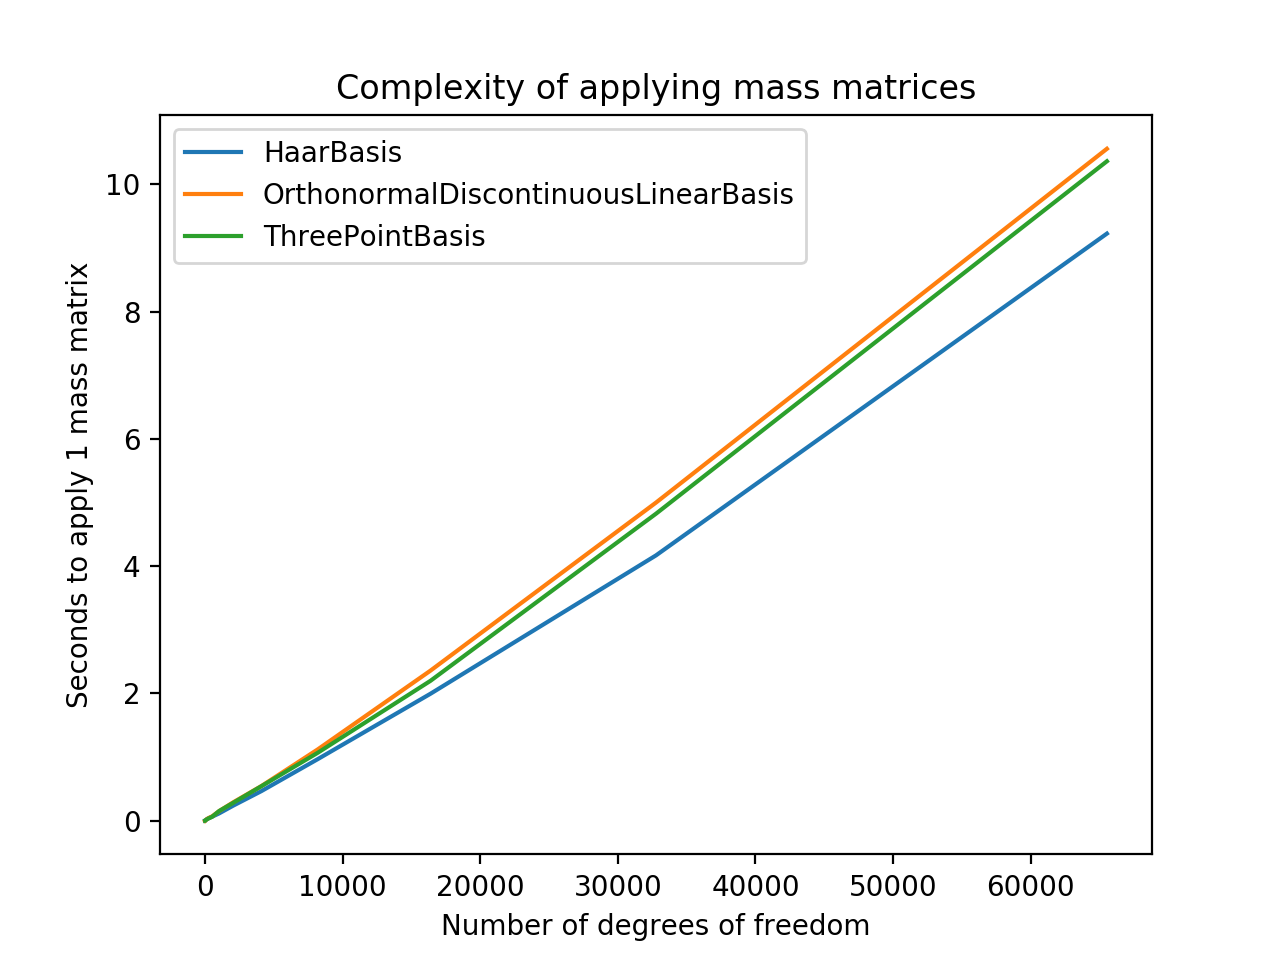
\includegraphics[width=0.5\linewidth]{../../Latex/img/time-scaling-31-jul.png}\hfill
  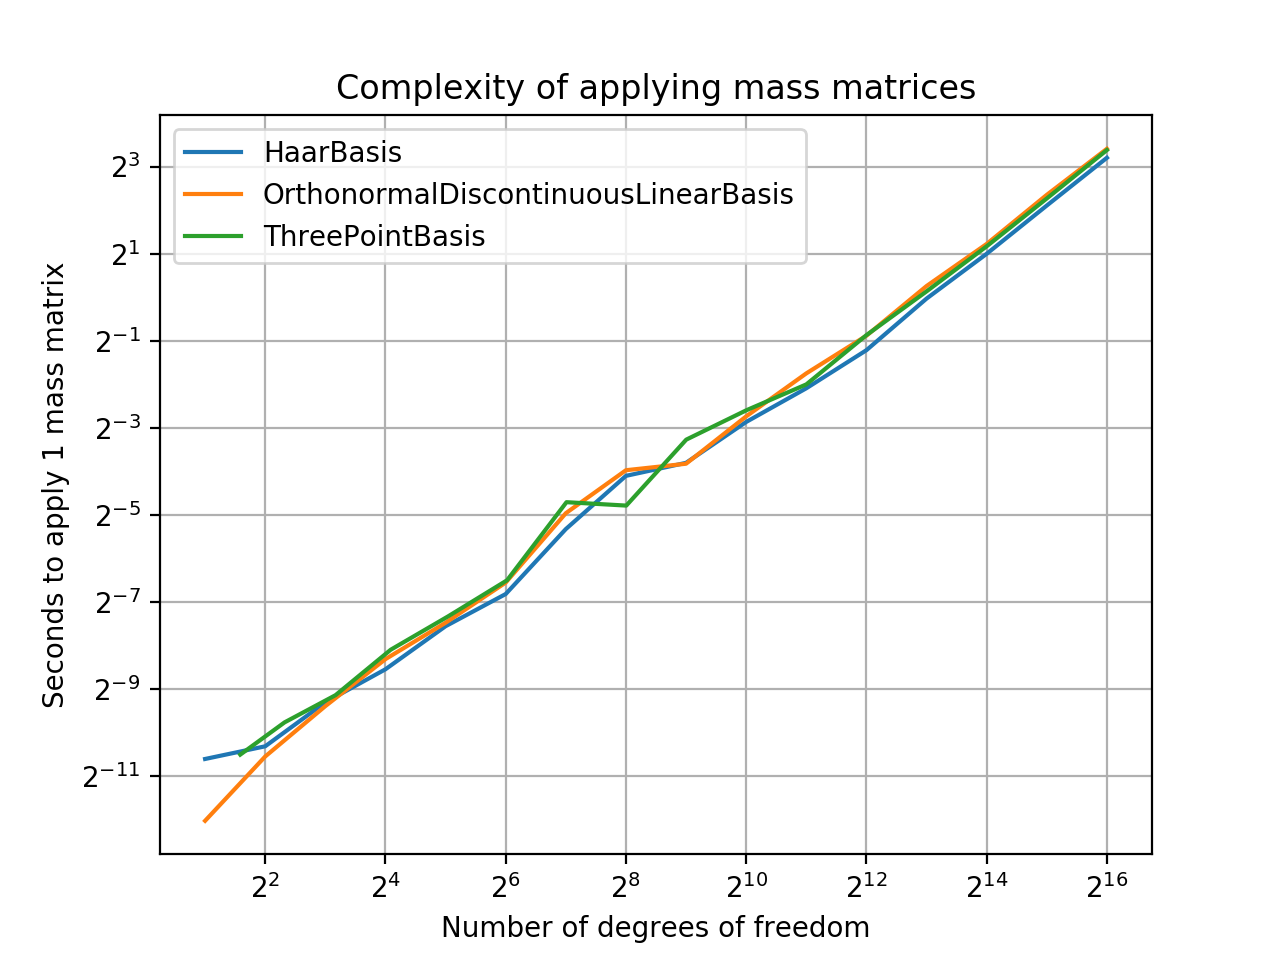
\includegraphics[width=0.5\linewidth]{../../Latex/img/time-scaling-31-jul-loglog.png}
  \caption{Wallclock time on my laptop for a single call to \texttt{apply()} on a uniform grid. Left: linear-linear plot; right: log-log plot.}
  \label{fig:linear}
\end{figure}
\subsection{Bottlenecks}
\begin{verbatim}
      ncalls  tottime percall filename:lineno(function)
(1)  8125836    4.824   0.000 indexed_vector.py:69(<genexpr>)
(2)     1760    3.394   0.005 interval.py:36(__init__)
(3)  8129028    3.009   0.000 {built-in method __new__ of type object at 0x10e3a2050}
(4)  2752510    2.600   0.000 {built-in method builtins.sum}
(5)     1368    2.293   0.002 indexed_vector.py:54(__add__)
(6)  8129028    2.229   0.000 <string>:1(__new__)
(7)  2752510    2.219   0.000 indexed_vector.py:67(dot)
(8)      880    2.135   0.012 applicator.py:147(<setcomp>)
(9)     1320    2.047   0.010 linear_operator.py:25(<dictcomp>)
     1965762    1.909   0.000 orthonormal_basis.py:105(scaling_support)
     2621416    1.889   0.000 interval.py:63(covers)
     3538994    1.845   0.000 interval.py:12(intersects)
     1965906    1.758   0.000 haar_basis.py:84(scaling_support)
(10)    1960    1.661   0.001 {built-in method builtins.sorted}
\end{verbatim}
Total runtime to produce the above graph was about 1 minute (57 sec total).
In the verbatim (creating using \texttt{cProfile}, see also \texttt{timing\_test.py},
we see that there are no very obvious bottlenecks. Nonetheless, let's discuss some
of the things we see (NB: there are numbers in the left-hand side of some lines of the verbatim; they correspond with numbers below).

\begin{enumerate}
  \item Most of the time is spent doing dot products, as can be seen from the code:
    \begin{verbatim}
69  return sum(self.vector[labda] * other[labda] for labda in other.keys()
70             if labda in index_mask)\end{verbatim}
    I am not sure we can do much about this. It makes sense to do it, I think.
  \item We spend a lot of time merging these intervals, probably for constructing
    $\Pi_B$ and $\underline \Pi$. If we think some more about optimizing these
    calls, this will probably go away.
  \item This is a little cryptic but is about creating \texttt{Interval} objects.
    As we are not really doing much with them, possibly it would be better to
    just use \texttt{tuple}s in a next iteration.
  \item This is again to produce the dot-product; see snippet above.
  \item We are lazy and append two disjoint vectors by just adding them; this
    could maybe be improved.
  \item This has to do with creating \texttt{Interval} objects, I think this line
    is because \texttt{Interval} inherits from \texttt{collections.namedtuple}
    which is supposed to be faster than a regular \texttt{object}.
  \item More dot-product business.
  \item This is where we compute $\underline \Pi$, through
    \begin{verbatim}
145  ivs = IntervalSet([basis.scaling_support(index) for index in Pi_B] +
146                    [basis.wavelet_support(index) for index in Lambda_l])
147  return SingleLevelIndexSet({
148      index
149      for index in basis.scaling_indices_on_level(l)
150      if ivs.covers(basis.scaling_support(index))
151  })\end{verbatim}
    as you can see, every call to this is quite expensive. This is because the
    size of $\Delta_\ell$ grows exponentially in $\ell$.\footnote{Actually, for
    nonuniform grids, a much smaller set can be used, but \texttt{haar\_basis.py}
    and \texttt{orthonormal\_basis.py} contain two TODO's in this direction.}
  \item This is overhead of allocating new \texttt{IndexedVector}s at every
    matvec. We could opt to do most matvecs in-place (by passing an
    \texttt{out}-argument).
  \item One can see that only 1.6 seconds is spent sorting, even though quite a
    lot of our (nonoptimized) code uses sorting. This is nice.
\end{enumerate}

\subsection{Caveat on the 3-point basis}
So I (more or less blindly) implemented the basis. But the multiscale mass matrix
is not at all very sparse or something, which implies that these `wavelets' are
not $L_2([0,1])$-orthogonal to one another. I am not completely sure if this was
the goal of the basis, because if so, I have likely misunderstood something.
\emph{Still, we can apply the matrix in linear time even though it has $\mathcal O(N^2)$
elements :).}

\section{Towards tensor-product operators}
Before we can do things in space-time, a small number of things have to be fixed,
or at least looked at, in the time-code. They are marked with TODO, so
\texttt{grep -rI "TODO" .} should point you in the right directions.

In any case, right now, 


\end{document}
